% Cover, title page and credits page.
% The cover image is computed by code/cover.py (Voronoi cells of the triangular lattice); it carries no text.
\thispagestyle{empty}
\begin{tikzpicture}[remember picture,overlay]
  \node[inner sep=0pt] at (current page.center)
    {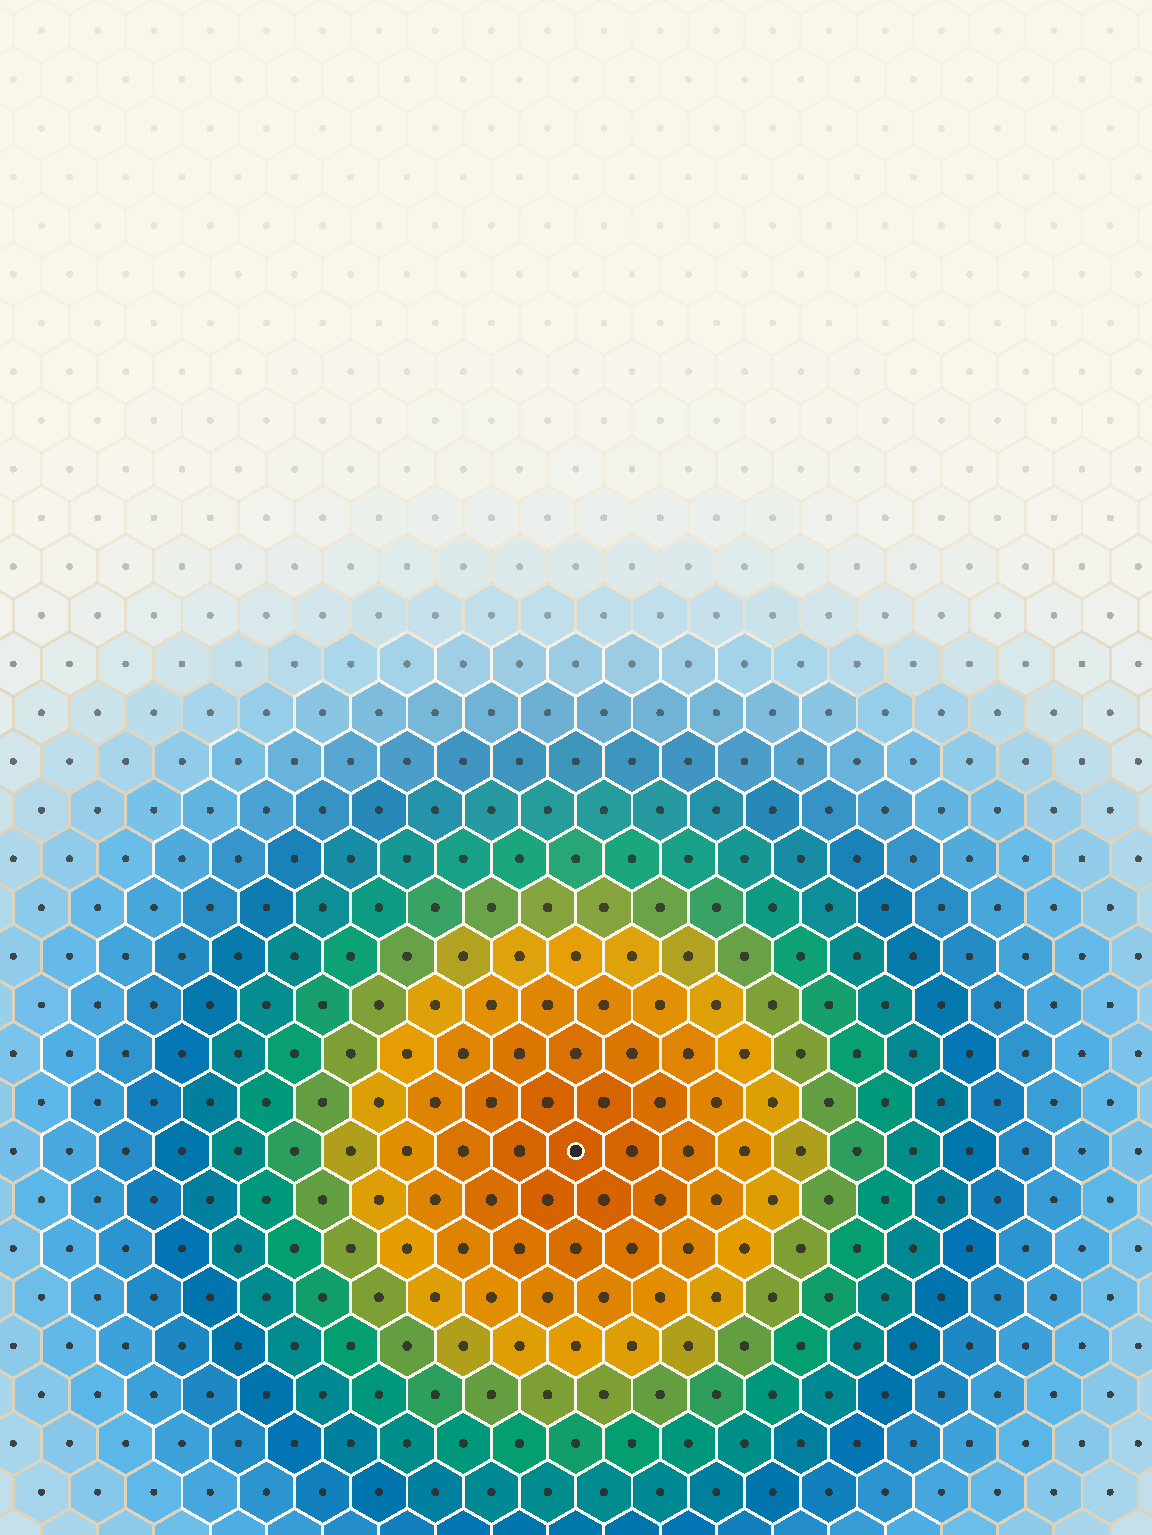
\includegraphics[width=\paperwidth,height=\paperheight]{cover.pdf}};
  \node[anchor=north west,inner sep=0pt,text width=15.2cm,align=left]
    at ([xshift=2.1cm,yshift=-3.0cm]current page.north west) {%
    {\sffamily\bfseries\footnotesize\color{okbleu}\textls[200]{XAVIER CALLENS}}\\[1.1cm]
    {\fontsize{40}{44}\selectfont\color{encre}The\hspace{0.3em}Discovery\\[2pt] Journal}\\[0.8cm]
    {\color{okorange}\rule{3.2cm}{1.6pt}}\\[0.55cm]
    {\fontsize{13.5}{18}\selectfont\itshape\color{encre!85}A year in which AI proposes, the computer calculates,\\
      the proof judges and humans decide what it means}};
  \node[anchor=south west,inner sep=0pt,text width=15cm,align=left]
    at ([xshift=2.1cm,yshift=1.6cm]current page.south west) {%
    {\sffamily\footnotesize\bfseries\color{ivoire}\textls[160]{SOCRATEAI LAB}}};
\end{tikzpicture}
\clearpage
% back of the cover
\thispagestyle{empty}
\vspace*{\fill}
\begin{adjustwidth}{0pt}{-3cm}
\noindent{\footnotesize\color{encre!70}\textit{The cover.} Each hexagon is the Voronoi cell of one point of the
triangular lattice of density~1: the set of places in the plane that are closer to that point than to any other.
All these cells have exactly the same area, equal to~1. The colour of a cell gives the weight
$e^{-\pi\alpha r^2}$, with $\alpha=0.009$, of its point in the energy of the central point (the black dot), where $r$
is the distance between them: vermilion and orange close by, then green and blue, ivory far away. The picture is
computed, not drawn by hand (\texttt{code/cover.py}); the program checks that every cell really has six sides and an
area of~1, and that a slightly deformed lattice fails this test.}
\end{adjustwidth}
\clearpage

% title page
\thispagestyle{empty}
\vspace*{2.2cm}
{\sffamily\bfseries\footnotesize\color{okbleu}\textls[200]{XAVIER CALLENS}}\par
\vspace{1.4cm}
{\fontsize{34}{38}\selectfont The\hspace{0.3em}Discovery\hspace{0.3em}Journal\par}
\vspace{0.6cm}
{\color{okorange}\rule{3.2cm}{1.6pt}}\par
\vspace{0.5cm}
{\large\itshape A year in which AI proposes, the computer calculates,\\ the proof judges and humans decide what it
means\par}
\vspace{1.4cm}
{\normalsize Twenty contributions in mathematics, physics, genetics and cosmology,\\
told in plain words, with their limits and their mistakes\par}
\vspace*{\fill}
{\sffamily\footnotesize\color{encre!80}\textls[120]{SOCRATEAI LAB}\quad·\quad\lfstyle English edition, version 1,
October 2026\par}
\clearpage

% back of the title page: credits and statement on AI
\thispagestyle{empty}
\vspace*{\fill}
\begin{adjustwidth}{0pt}{-2cm}
\small
\noindent\textbf{The Discovery Journal.} A year in which AI proposes, the computer calculates, the proof judges and
humans decide what it means.\par\medskip
\noindent Xavier Callens, SocrateAI Lab. English edition, version 1, October 2026. DOI: 10.5281/zenodo.23669463. It is the English edition of \textit{Le journal des découvertes} (DOI: 10.5281/zenodo.23669395), translated from the French by artificial
intelligence agents under the author's direction.\par\medskip
\noindent\textbf{Statement on artificial intelligence.} This book was written with artificial intelligence agents
(Claude, by Anthropic), under the direction of the author, who chose its subject, its plan and its tone, and who is
responsible for it. The results it tells were also produced by AI agents under the author's direction, and then
audited by other AI agents. \textbf{No human mathematician has reviewed them.} Several of them depend on theorems
published by openai/math, which were also produced by an AI and have not yet been peer reviewed. Every claim carries
a confidence level (A, As, L, C or X), explained in Chapter~1.\par\medskip
\noindent\textbf{Sources.} The facts and numbers in this book come from the records of the work itself
(Zenodo, GitHub) and from the selection file described at the end of the book (``How this book was made''). A number
that does not appear there is not used.\par\medskip
\noindent\textbf{Typesetting.} \LaTeX{} (pdflatex), Cochineal and Source Sans Pro typefaces, Okabe--Ito colour
palette, chosen because it stays readable for colour-blind readers. The figures are computed by programs from the
real numbers.
\end{adjustwidth}
\vspace*{1.5cm}
\clearpage
